\documentclass[aspectratio=169, 14pt]{beamer}
\input{preamble}

\title{Large Language Models}
\subtitle{A Physicist's Perspective}
\date{Physikalisches Kolloquium, Universit\"at W\"urzburg, 13 July 2026}

% --- Placeholder caption for the unit-distance hook (patch later) ---
\newcommand{\unitdistancecaption}{%
  arXiv:2605.20695 \quad\textperiodcentered\quad
  Alon, Bloom, Gowers, Litt, Sawin, Shankar, Tsimerman, Wang, Matchett Wood
  \quad\textperiodcentered\quad May 2026\\[2pt]
  human verification of an OpenAI-generated counterexample}

% --- Reusable grey honesty caption for the synthetic grade figures ---
\newcommand{\synthcaption}{%
  {\small\color{tjo@black!55}%
   Synthetic data, illustrative: reproduces the structure of the
   real six-year analysis.}}

\begin{document}

% =====================================================================
% TITLE
% =====================================================================

\begin{frame}[plain]
  \titlepage
\end{frame}

% =====================================================================
% PART 1: WHY THIS TALK?
% =====================================================================

\sectiondivider{Why this talk?}

% --- Hook A: unit-distance problem (asset produced in parallel) ---
\begin{frame}[plain]
  \vfill
  \centering
  \IfFileExists{assets/unitdistance_pr.png}{%
    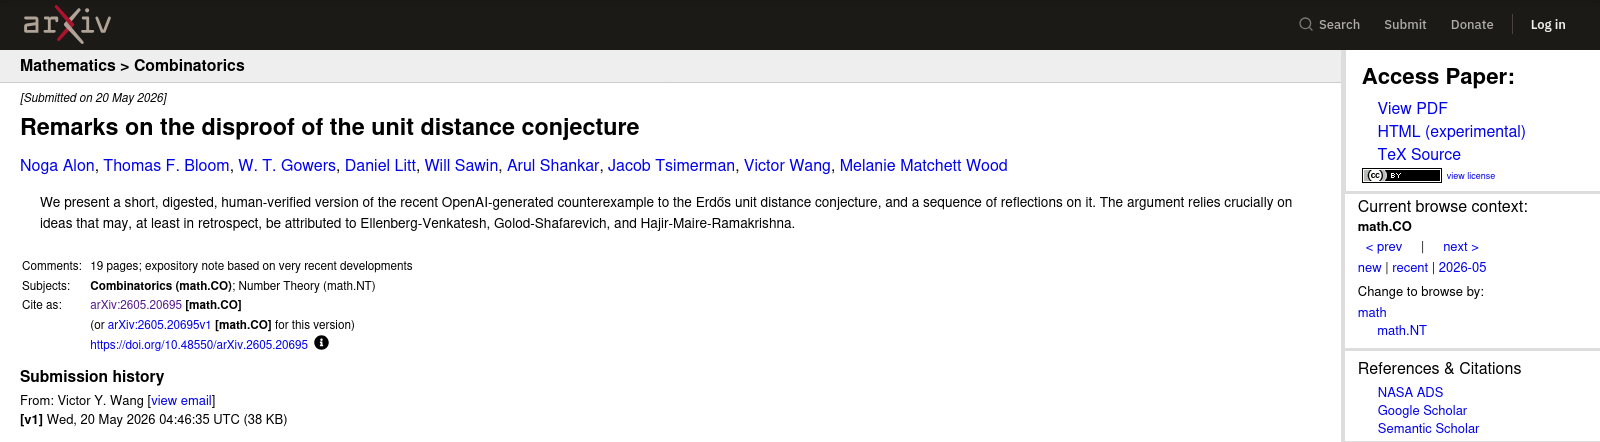
\includegraphics[width=0.82\textwidth]{assets/unitdistance_pr.png}%
  }{%
    % SPEC-DEVIATION: asset is being produced in parallel; show a
    % visible placeholder so the deck always compiles.
    \begin{tikzpicture}
      \draw[tjo@darkteal, line width=1.5pt, rounded corners=6pt]
        (0,0) rectangle (10,5.6);
      \node[align=center, text=tjo@black!55, font=\large] at (5,2.8)
        {\textbf{[ assets/unitdistance\_pr.png ]}\\[0.6em]
         full-bleed press screenshot\\ (produced in parallel)};
    \end{tikzpicture}%
  }

  \vskip1em
  {\small\color{tjo@black!60}\unitdistancecaption}
  \vfill
\end{frame}

% --- Hook B: OpenAI string-theory paper (verbatim from GC deck) ---
\begin{frame}[plain]
  \vfill
  \centering
  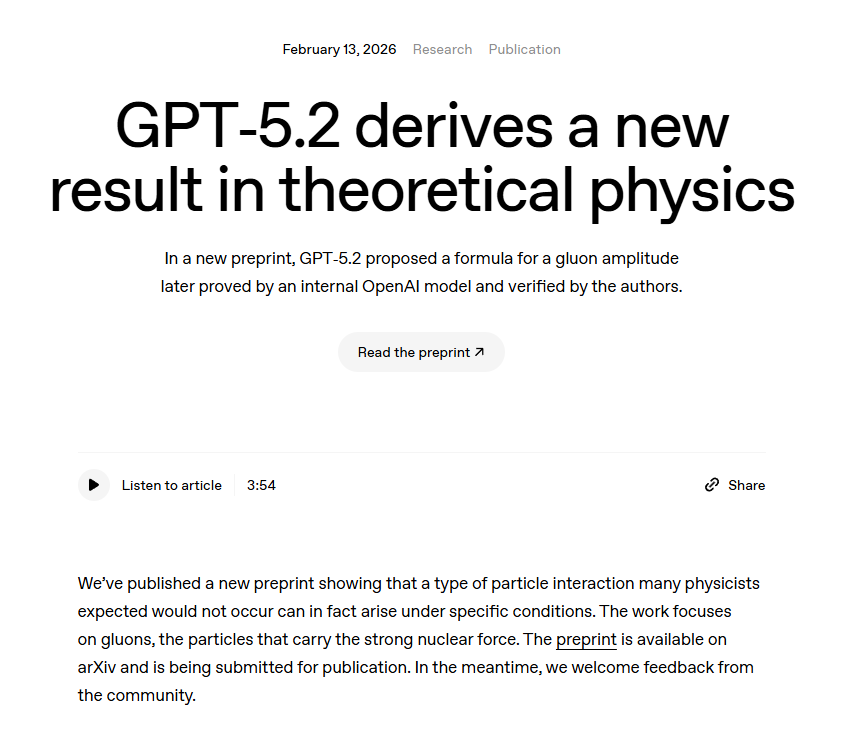
\includegraphics[width=0.68\textwidth]{assets/gpt52pr.PNG}

  \vskip0.8em
  {\small\color{tjo@black!60}%
    arXiv:2602.12176 \quad\textperiodcentered\quad
    IAS, Harvard, Cambridge, Vanderbilt, OpenAI \quad\textperiodcentered\quad
    February 2026}
  \vfill
\end{frame}

% --- Hook C1: grade decorrelation --- a control experiment run on us ---
\begin{frame}{A control experiment, run on us}
  \begin{flushleft}
  \hspace{1.5em}First-year theoretical physics, six years of grades

  \vskip0.5em
  \hspace{1.5em}Weekly take-home assignment, out of 100
  {\color{tjo@black!55} (unsupervised)}

  \vskip0.5em
  \hspace{1.5em}Invigilated final exam, out of 10
  {\color{tjo@black!55} (the control)}

  \vskip0.5em
  \hspace{1.5em}2020--2023: the two agree at $b \approx 0.10$
  \end{flushleft}

  \vskip0.8em
  \centering
  {\color{tjo@darkteal}\bfseries
    When the link breaks, it is the assignment that broke, not the exam}

  \vskip0.6em
  \synthcaption
\end{frame}

% --- Hook C2: 2020 baseline ---
\begin{frame}{2020: the instruments agree}
  \centering
  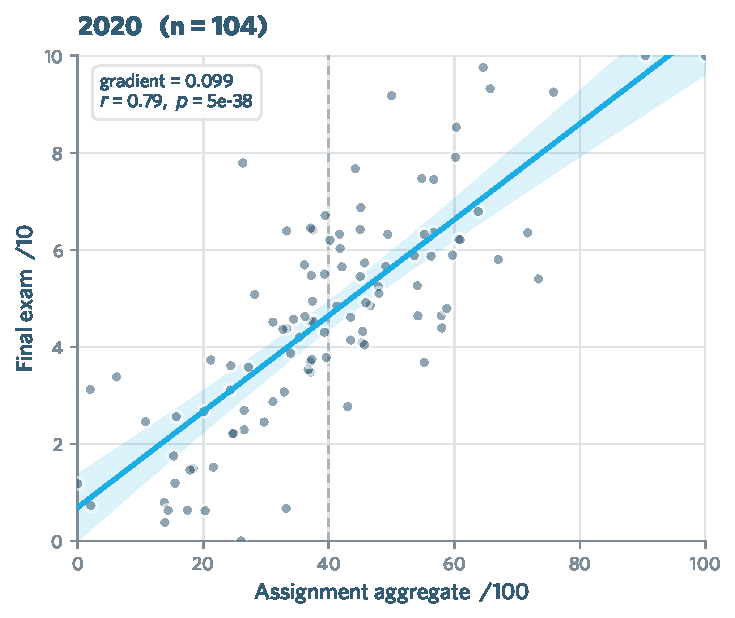
\includegraphics[height=0.52\textheight]{../grade-decorrelation/figures/scatter_2020.pdf}

  \vskip0.4em
  {\small\color{tjo@darkteal}\bfseries
    $b = 0.099$, $r = 0.79$:} {\small the assignment predicts the exam}

  \vskip0.3em
  \synthcaption
\end{frame}

% --- Hook C3: 2025 collapse ---
\begin{frame}{2025: the link is gone}
  \centering
  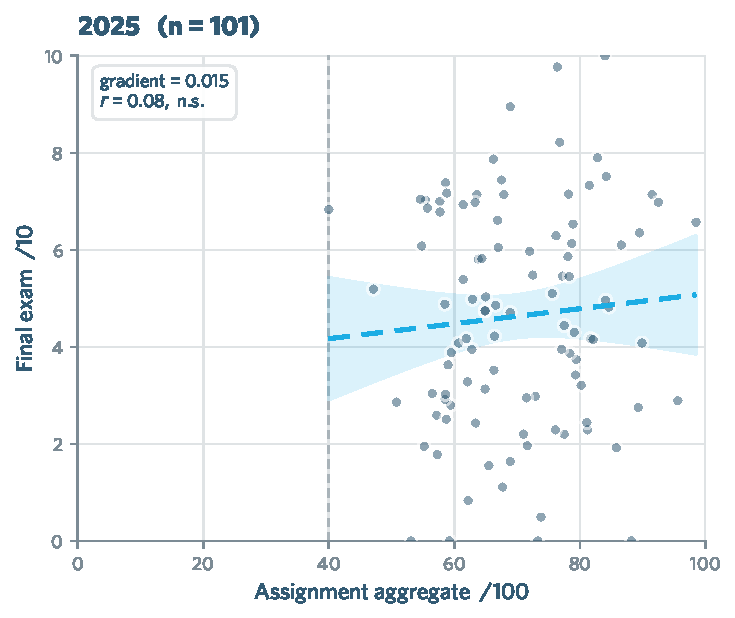
\includegraphics[height=0.52\textheight]{../grade-decorrelation/figures/scatter_2025.pdf}

  \vskip0.4em
  {\small\color{tjo@darkteal}\bfseries
    $b = 0.015$, $r = 0.08$, n.s.:} {\small it no longer measures what the
  exam measures}

  \vskip0.3em
  \synthcaption
\end{frame}

% --- Hook C4: the collapse in one image (punchline) ---
\begin{frame}{The collapse, one panel per year}
  \centering
  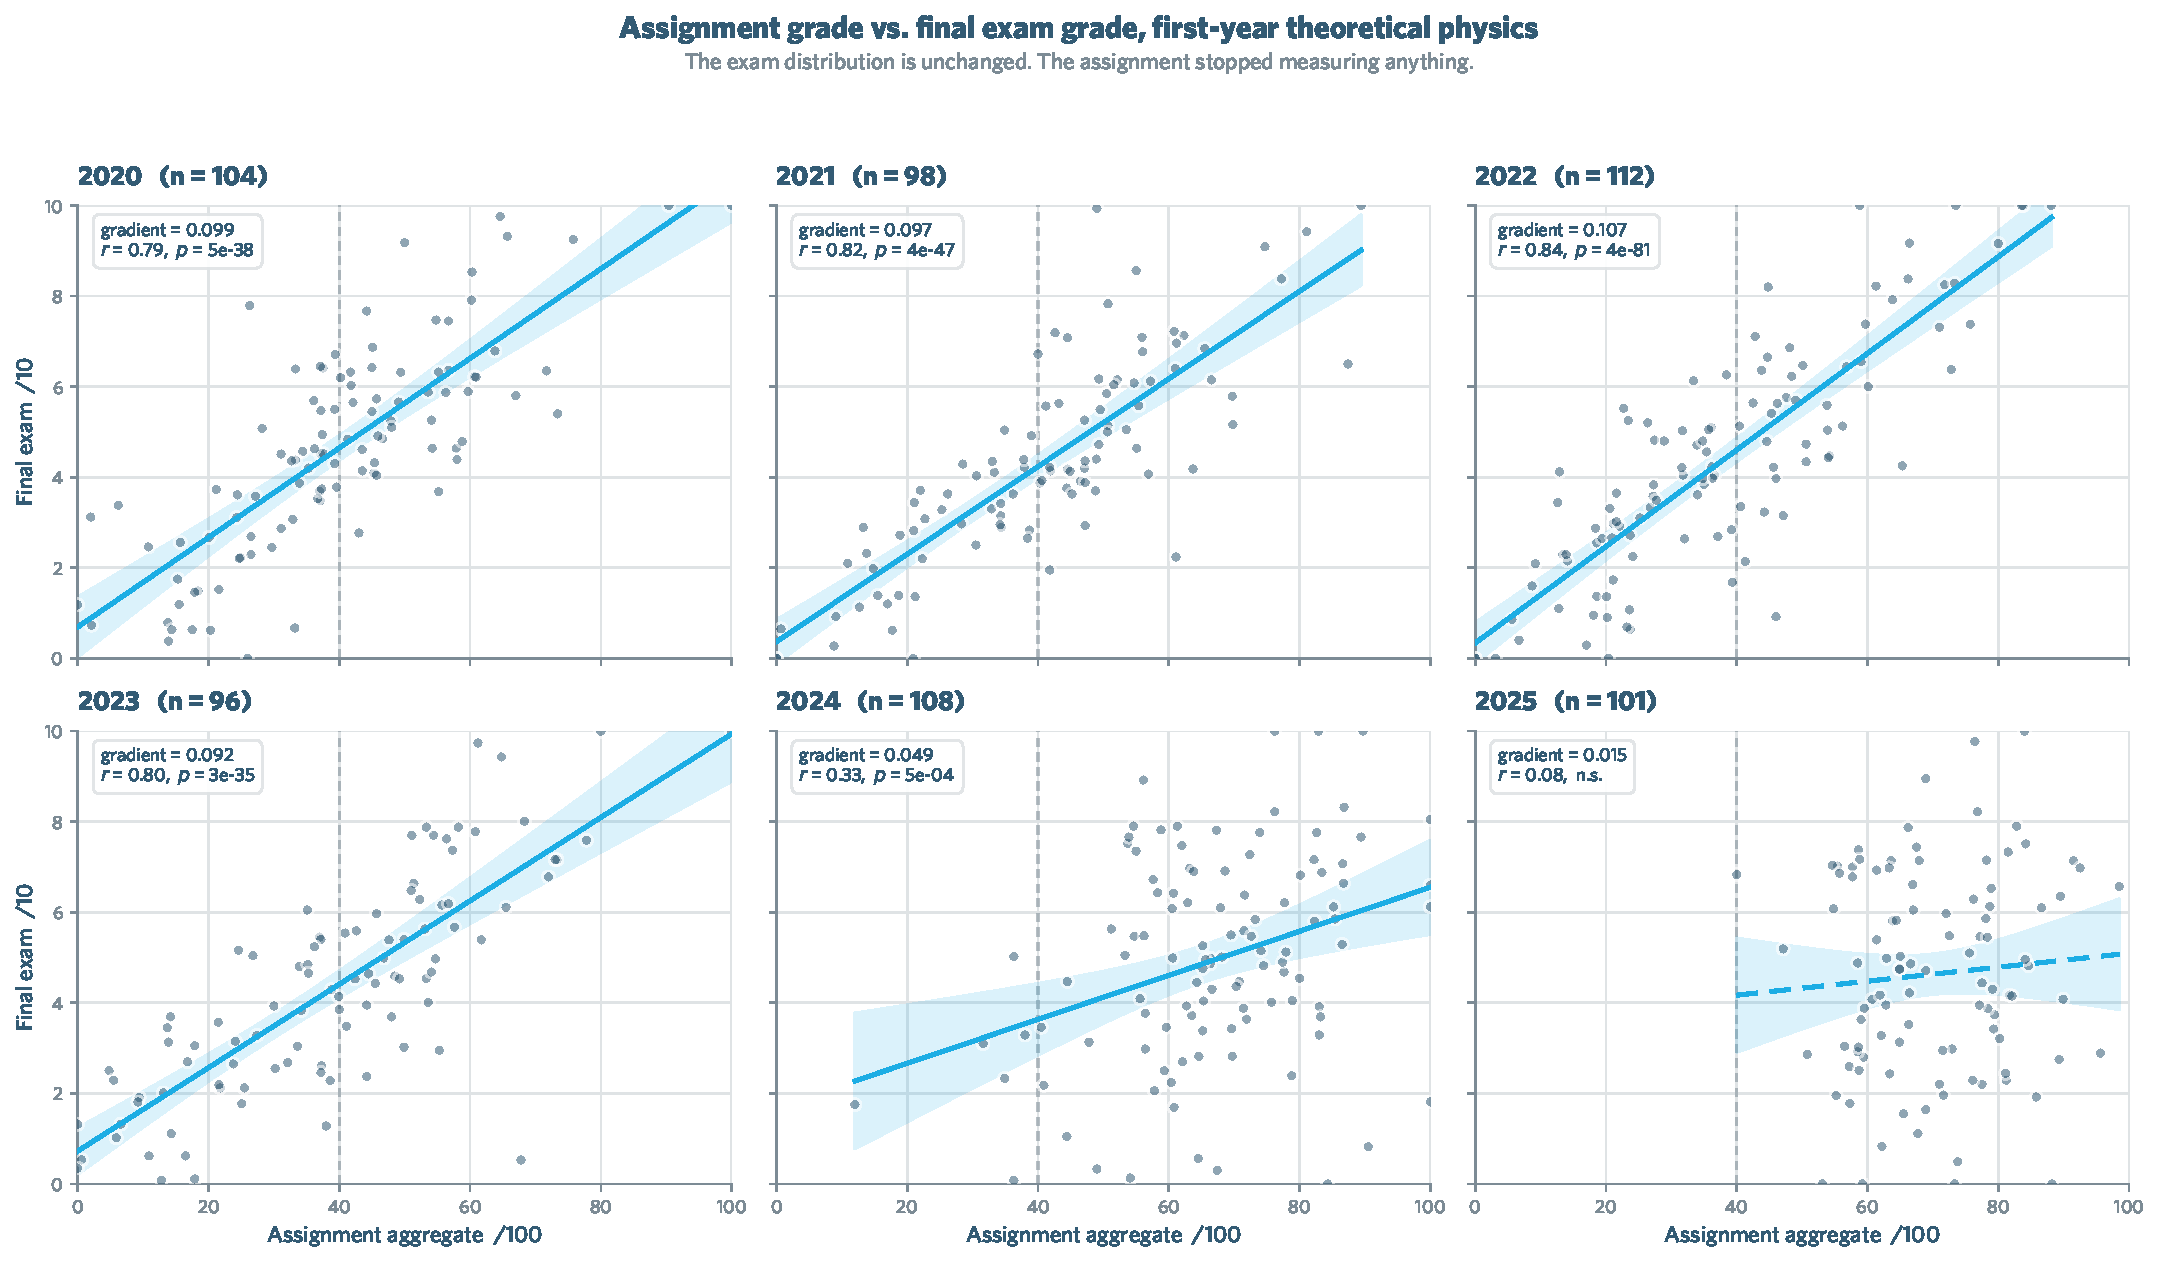
\includegraphics[height=0.40\textheight]{../grade-decorrelation/figures/scatter_grid.pdf}

  \vskip0.2em
  {\footnotesize\color{tjo@darkteal}\bfseries
    Pooled interaction $d = -0.063$, $p \approx 1\times10^{-7}$:} {\footnotesize
  adoption is uncorrelated with ability}

  \vskip0.15em
  \synthcaption
\end{frame}

% --- Audience survey (adapted from seminar deck) ---
\begin{frame}{Quick survey: hands up}
  \vfill
  \centering
  {\fontsize{20}{30}\selectfont
    \begin{tabular}{l}
      \color{tjo@cyan}$\bullet$\quad Who has used ChatGPT, Claude, or Gemini? \\[0.9em]
      \color{tjo@cyan}$\bullet$\quad Who has used one for research? \\[0.9em]
      \color{tjo@cyan}$\bullet$\quad Who has used a coding agent? \\
    \end{tabular}
  }
  \vfill
\end{frame}

% --- Timeline: four moments (extends GC deck's three-moment timeline) ---
\begin{frame}{Four moments}
  \vfill
  \centering
  \begin{tikzpicture}[
    event/.style={
      tjo box,
      minimum width=2.7cm,
      minimum height=1.7cm,
      font=\footnotesize,
      align=center,
    },
  ]
    \draw[tjo@black!20, line width=2pt] (-6.7,0) -- (6.7,0);

    \node[event, fill=tjo@lightgrey] at (-5.2,0) {%
      {\bfseries\small\color{tjo@darkteal} Nov 2022}\\[3pt]
      ChatGPT\\launches
    };
    \node[event, fill=tjo@lightgrey] at (-1.7,0) {%
      {\bfseries\small\color{tjo@darkteal} Q1 2025}\\[3pt]
      Claude Code,\\Cursor, Copilot
    };
    \node[event, fill=tjo@lightgrey] at (1.7,0) {%
      {\bfseries\small\color{tjo@darkteal} Q4 2025}\\[3pt]
      Opus 4.5, GPT-5.2\\cross a threshold
    };
    \node[event, fill=tjo@cyan!25] at (5.2,0) {%
      {\bfseries\small\color{tjo@darkteal} Q2 2026}\\[3pt]
      Fable 5, GPT-5.6,\\GLM-5.2
    };
  \end{tikzpicture}
  \vfill
\end{frame}

% --- Capable but untrustworthy (verbatim, GC deck) ---
\statementslide{LLMs are \textbf{incredibly capable}\\[0.5em]
  but \textbf{maximally untrustworthy}}

% --- The gap (verbatim, GC deck) ---
\begin{frame}[plain,c]
  \centering
  {\fontsize{22}{30}\selectfont\color{tjo@darkteal}
    The gap between\\[0.6em]
    {\bfseries ``I tried ChatGPT and it hallucinated''}\\[0.6em]
    and\\[0.6em]
    {\bfseries ``this is a powerful force multiplier''}\\[0.8em]
  }
  {\fontsize{20}{26}\selectfont\color{tjo@darkteal}
    is not closed by better models\\[0.5em]
    It is closed by \textbf{technique} and \textbf{domain expertise}
  }
\end{frame}

% =====================================================================
% PART 2: WHAT IS AN LLM?
% =====================================================================

\sectiondivider{What is an LLM?}

% --- A new kind of resource ---
\begin{frame}[plain,c]
  \centering
  {\fontsize{22}{30}\selectfont\color{tjo@darkteal}\bfseries
    A new kind of resource:\\[0.5em]
    general-purpose intelligence,\\[0.3em]
    bought by the token}

  \vskip1.2em
  {\fontsize{18}{24}\selectfont\color{tjo@black!55}(somewhat)}
\end{frame}

% --- From outside, looking in (GC deck) ---
\begin{frame}[fragile]{From outside, looking in}
  \vfill
\begin{codeblock}
f : String -> String
\end{codeblock}
  \vskip1.5em
  \begin{flushleft}
  \hspace{1.5em}Outside the API boundary, this is the observable behaviour

  \medskip
  \hspace{1.5em}No hidden state is carried between calls
  \end{flushleft}
  \vfill
\end{frame}

% --- Nondeterministic (GC deck) ---
\begin{frame}{Nondeterministic}
  \vfill
  \centering
  \begin{tikzpicture}
    \node[tjo box fill, minimum width=3.5cm, font=\normalsize] (input) {\texttt{"What is spin?"}};

    \node[tjo box, right=4cm of input, yshift=1.5cm, font=\normalsize]  (o1) {\texttt{"Spin is\ldots"}};
    \node[tjo box, right=4cm of input, font=\normalsize]                 (o2) {\texttt{"Angular\ldots"}};
    \node[tjo box, right=4cm of input, yshift=-1.5cm, font=\normalsize] (o3) {\texttt{"In QM\ldots"}};

    \draw[tjo arrow] (input.east) -- (o1.west);
    \draw[tjo arrow] (input.east) -- (o2.west);
    \draw[tjo arrow] (input.east) -- (o3.west);
  \end{tikzpicture}

  \vskip0.8em
  {\normalsize Same input, different outputs:
  the model samples from $\Prob(\text{next token} \given \text{context})$}
  \vfill
\end{frame}

% --- Temperature / Boltzmann (GC deck) ---
\begin{frame}{Temperature}
  \vfill
  \[
    P(\text{token}_i) \;=\; \frac{\exp(\ell_i / T)}{\displaystyle\sum_j \exp(\ell_j / T)}
  \]

  \vskip1.5em
  \centering
  {\color{tjo@darkteal}\bfseries Direct analogy to the Boltzmann distribution}

  \vskip1em
  {\normalsize $T \to 0$: deterministic (ground state)
    \qquad $T \to \infty$: uniform (infinite temperature)}
  \vfill
\end{frame}

% --- Tokens (seminar deck) ---
\begin{frame}[fragile]{Tokens}
  \vfill
  Not characters. Not words.

  \medskip
  Subword chunks from a fixed vocabulary $V$ of ${\sim}100\text{k}$ entries.

  \vskip1.5em
\begin{codeblock}
'theoretical physics'  ->  ['theor', 'etical', ' physics']
\end{codeblock}

  \vskip1em
  {\small\color{tjo@black!60}
    More precisely: $f : \text{Token}^* \to \text{Token}^*$}
  \vfill
\end{frame}

% --- Closing definition (GC deck) ---
\begin{frame}[plain,c]
  \centering
  {\fontsize{18}{25}\selectfont\color{tjo@darkteal}
  An LLM is a stateless, nondeterministic function

  \vskip0.6em
  \[ f : \text{String} \to \text{String} \]

  \vskip0.6em
  that samples from $\Prob(\text{next\_token} \given \text{context})$

  \medskip
  via a single forward pass through a frozen neural network
  }
\end{frame}

% =====================================================================
% PART 3: THE ILLUSION OF CHAT
% =====================================================================

\sectiondivider{The illusion of chat}

% --- A single API call (cURL, seminar deck) ---
\begin{frame}[fragile]{A single API call}
\begin{codeblock}
curl https://api.anthropic.com/v1/messages \
  -H "x-api-key: $KEY" \
  -H "content-type: application/json" \
  -H "anthropic-version: 2023-06-01" \
  -d '{"model":"claude-sonnet-4-6", "max_tokens":256,
       "messages":[{"role":"user","content":"What is a quark?"}]}'
\end{codeblock}

  \vskip1em
  \centering
  {\large One string in, one string out: the entire interaction}
\end{frame}

% --- How chat works (seminar deck) ---
\begin{frame}[fragile]{How chat works}
  \vfill
\begin{codeblock}
Turn 1:  [user_1]
Turn 2:  [user_1, asst_1, user_2]
Turn 3:  [user_1, asst_1, user_2, asst_2, user_3]
\end{codeblock}

  \vskip1.5em
  \centering
  The client re-sends the \textbf{entire} history every turn:
  the LLM has no memory
  \vfill
\end{frame}

% --- The context window (GC merged version) ---
\begin{frame}{The context window}
  \vfill
  \centering
  \begin{tikzpicture}
    \fill[tjo@lightgrey] (0,0) rectangle (12,1.2);
    \fill[tjo@darkteal!30] (0,0) rectangle (2,1.2);
    \node[font=\small, text=tjo@darkteal, align=center] at (1,0.6) {system\\ prompt};
    \fill[tjo@cyan!20] (2,0) rectangle (9.5,1.2);
    \node[font=\small, align=center] at (5.75,0.6) {conversation history};
    \fill[tjo@cyan!40] (9.5,0) rectangle (12,1.2);
    \node[font=\small, align=center] at (10.75,0.6) {latest\\ message};
    \draw[tjo@darkteal, line width=1pt] (0,0) rectangle (12,1.2);
    \draw[decorate, decoration={brace, amplitude=8pt, mirror},
          tjo@darkteal, line width=1pt]
      (0,-0.3) -- (12,-0.3)
      node[midway, below=10pt, font=\normalsize] {context window (tokens)};
  \end{tikzpicture}

  \vskip1em
  Everything the model sees must fit here:
  from a few thousand tokens (free chat) to ${\sim}1$M (frontier)

  \vskip0.5em
  {\color{tjo@darkteal}\bfseries
    When the conversation exceeds it, something must be dropped}
  \vfill
\end{frame}

% --- Context rot (seminar deck) ---
\begin{frame}{Context rot}
  \vfill
  \begin{flushleft}
  \hspace{1.5em}As the context fills, older information gets buried

  \vskip1.2em
  \hspace{1.5em}The model's effective attention degrades

  \vskip1.2em
  \hspace{1.5em}Your constraints, instructions, and earlier results silently disappear
  \end{flushleft}

  \vskip1.5em
  \centering
  {\color{tjo@darkteal}\bfseries
    This is why chat interfaces silently ruin your results}
  \vfill
\end{frame}

% --- Compaction (NEW) ---
\begin{frame}{Compaction}
  \vfill
  \centering
  \begin{tikzpicture}
    % Full window
    \fill[tjo@cyan!20] (0,1.2) rectangle (11,2.0);
    \draw[tjo@darkteal, line width=1pt] (0,1.2) rectangle (11,2.0);
    \node[font=\small, align=center] at (5.5,1.6) {long conversation history (window full)};

    % Arrow down
    \draw[tjo arrow] (5.5,1.0) -- (5.5,0.3)
      node[midway, right, font=\small, text=tjo@darkteal] {summarise};

    % Compacted: small summary + fresh space
    \fill[tjo@darkteal!30] (0,-0.9) rectangle (2.4,-0.1);
    \node[font=\small, text=tjo@darkteal, align=center] at (1.2,-0.5) {summary};
    \fill[tjo@lightgrey] (2.4,-0.9) rectangle (11,-0.1);
    \node[font=\small, text=tjo@black!55, align=center] at (6.7,-0.5) {fresh space};
    \draw[tjo@darkteal, line width=1pt] (0,-0.9) rectangle (11,-0.1);
  \end{tikzpicture}

  \vskip1.2em
  Lossy by construction: you do not control what survives

  \vskip0.5em
  {\color{tjo@darkteal}\bfseries
    Chat interfaces do this silently; this is why long chats go off the rails}
  \vfill
\end{frame}

% =====================================================================
% PART 4: FROM FUNCTION TO AGENT
% =====================================================================

\sectiondivider{From function to agent}

% --- The agent loop (code, GC deck) ---
\begin{frame}[fragile]{The agent loop}
  \vfill
\begin{codeblock}
while not done:
    response = llm(system_prompt + history)
    tool_calls = parse(response)
    results = execute(tool_calls)
    history += [response, results]
\end{codeblock}

  \vskip1.5em
  \centering
  {\color{tjo@darkteal}\bfseries
    This is the complete architecture of every coding agent}
  \vfill
\end{frame}

% --- The agent loop (diagram, GC deck) ---
\begin{frame}{The agent loop}
  \vfill
  \centering
  \begin{tikzpicture}[node distance=1.6cm, every node/.style={align=center}]
    \node[tjo box, fill=tjo@darkteal, text=white, minimum width=4cm,
          minimum height=1cm, font=\normalsize]
      (sys) {System prompt + History};

    \node[tjo box fill, below=1.2cm of sys, minimum width=4cm,
          minimum height=1cm, font=\normalsize]
      (llm) {\textbf{LLM}\; {\small\code{f(s) $\to$ s}}};

    \node[tjo box, right=3cm of llm, minimum height=1cm, font=\normalsize]
      (parse) {Parse tool calls};

    \node[tjo box, below=1.2cm of parse, minimum height=1cm, font=\normalsize]
      (exec) {Execute tools};

    \draw[tjo arrow] (sys) -- (llm);
    \draw[tjo arrow] (llm) -- (parse)
      node[midway, above, font=\small] {response};
    \draw[tjo arrow] (parse) -- (exec)
      node[midway, right, font=\small] {call};

    \draw[tjo arrow] (exec.south) -- ++(0,-0.6) -| ([xshift=-0.5cm]llm.south)
      node[near start, below, font=\small] {results};

    \draw[tjo arrow, dashed, color=tjo@cyan]
      ([xshift=0.5cm]llm.north) -- ([xshift=0.5cm]sys.south)
      node[midway, right, font=\small, text=tjo@cyan] {append};
  \end{tikzpicture}
  \vfill
\end{frame}

% --- The key insight (statement, GC deck) ---
\statementslide{The LLM never executes anything\\[0.8em]
  {\fontsize{20}{26}\selectfont\mdseries
    It generates text; your scaffolding acts on it}}

% --- Feedback stabilises: closing the loop (NEW) ---
\begin{frame}{Closing the loop}
  \vfill
  \centering
  \begin{tikzpicture}[every node/.style={align=center}]
    % Open loop
    \node[tjo box, minimum width=3.6cm, minimum height=1.4cm, font=\small] (chat)
      at (-4,0) {\textbf{Chat}\\[3pt]{\small open loop}\\[2pt]
        {\color{red!70!black}errors compound}};
    % Closed loop
    \node[tjo box fill, minimum width=3.6cm, minimum height=1.4cm, font=\small] (agent)
      at (4,0) {\textbf{Agent}\\[3pt]{\small closed loop}\\[2pt]
        {\color{tjo@darkteal}errors correct}};

    \draw[tjo arrow, line width=2pt] (chat.east) -- (agent.west)
      node[midway, above=8pt, font=\footnotesize, text=tjo@black!60] {tool results feed back};
  \end{tikzpicture}

  \vskip1.2em
  \begin{flushleft}
  \hspace{1.5em}A tool result flows straight back into the context

  \vskip0.6em
  \hspace{1.5em}A failing test, a stack trace, a wrong number: each becomes the next correction
  \end{flushleft}

  \vskip1em
  \centering
  {\color{tjo@darkteal}\bfseries
    Feedback stabilises an otherwise unstable system}
  \vfill
\end{frame}

% --- Filesystem = permanent memory (NEW, core claim) ---
\begin{frame}{The filesystem is permanent memory}
  \vfill
  \centering
  \begin{tikzpicture}[every node/.style={align=center}]
    \node[tjo box, minimum width=5cm, minimum height=2.4cm, font=\small] (chat)
      at (-3.4,0) {%
      {\bfseries\normalsize\color{tjo@darkteal} Chat}\\[6pt]
      context is the only state\\[3pt]
      it evaporates when the\\ window fills\\[3pt]
      {\color{red!70!black} rots, cannot be checked}};

    \node[tjo box fill, minimum width=5cm, minimum height=2.4cm, font=\small] (agent)
      at (3.4,0) {%
      {\bfseries\normalsize\color{tjo@darkteal} Agent}\\[6pt]
      the filesystem is the state\\[3pt]
      it survives the context\\ window\\[3pt]
      {\color{tjo@darkteal} persistent, checkable, versioned}};
  \end{tikzpicture}

  \vskip1em
  \begin{flushleft}
  \hspace{1.0em}(i) Memory that outlives the context window \quad
  (ii) ground truth the model can \emph{re-read} instead of half-remembering
  \end{flushleft}

  \vskip0.6em
  \centering
  {\color{tjo@darkteal}\bfseries The radical unlock versus chat}
  \vfill
\end{frame}

% --- Subagents (adapted from GC multi-agent slide) ---
\begin{frame}{Subagents}
  \vfill
  \centering
  \begin{tikzpicture}[node distance=1.6cm, every node/.style={align=center}]
    \node[tjo box, fill=tjo@darkteal, text=white,
          minimum width=5cm, minimum height=1cm, font=\normalsize]
      (sup) {\textbf{Supervisor}\\{\small delegates \& composes reports}};

    \node[tjo box fill, below left=1.3cm and 1cm of sup,
          minimum width=3.5cm, font=\normalsize]
      (a1) {\textbf{Worker}\\{\small fresh context}};
    \node[tjo box fill, below=1.3cm of sup,
          minimum width=3.5cm, font=\normalsize]
      (a2) {\textbf{Worker}\\{\small fresh context}};
    \node[tjo box fill, below right=1.3cm and 1cm of sup,
          minimum width=3.5cm, font=\normalsize]
      (a3) {\textbf{Worker}\\{\small fresh context}};

    \draw[tjo arrow] (sup) -- (a1) node[midway, left, font=\small] {task};
    \draw[tjo arrow] (sup) -- (a2);
    \draw[tjo arrow] (sup) -- (a3);

    \draw[tjo arrow, dashed, color=tjo@cyan] (a1.north) to[bend left=15] (sup.south west);
    \draw[tjo arrow, dashed, color=tjo@cyan] (a3.north) to[bend right=15] (sup.south east);
  \end{tikzpicture}

  \vskip0.6em
  Each worker gets a clean window; results return as short reports

  \vskip0.3em
  {\color{tjo@darkteal}\bfseries Context isolation is the point}
  \vfill
\end{frame}

% --- Adversarial verification (GC deck) ---
\begin{frame}{Adversarial verification}
  \vfill
  \centering
  \begin{tikzpicture}[node distance=2cm, every node/.style={align=center}]
    \node[tjo box fill, minimum width=3cm] (prover) {%
      \textbf{Prover}\\{\small constructs}};
    \node[tjo box fill, right=2cm of prover, minimum width=3cm] (verifier) {%
      \textbf{Verifier}\\{\small attacks}};
    \node[tjo box, fill=tjo@darkteal, text=white,
          right=2cm of verifier, minimum width=3cm] (formal) {%
      \textbf{Formaliser}\\{\small Lean proof}};

    \draw[tjo arrow] (prover) -- (verifier);
    \draw[tjo arrow] (verifier) -- (formal);
    \draw[tjo arrow, dashed, color=tjo@cyan, bend right=30]
      (verifier.north) to node[above, font=\small, text=tjo@cyan] {reject} (prover.north);
  \end{tikzpicture}

  \vskip1.5em
  {\color{tjo@darkteal}\bfseries
    Natural language is an inadequate verification mechanism}

  \vskip0.5em
  {\small\color{tjo@black!60} Formal proof = compiler for mathematics}
  \vfill
\end{frame}

% =====================================================================
% PART 5: LIVE DEMO
% =====================================================================

\sectiondivider{Live demo}

\begin{frame}[plain,c]
  \centering
  {\fontsize{30}{38}\selectfont\color{tjo@darkteal}\bfseries
    Let's try something}

  \vskip0.8em
  {\fontsize{20}{26}\selectfont\color{tjo@darkteal} (no promises)}

  \vskip1.6em
  {\fontsize{16}{22}\selectfont\color{tjo@black!60}
    The prompt is pre-written; paste it into Claude Code}
\end{frame}

% =====================================================================
% PART 6: THE TREND
% =====================================================================

\sectiondivider{The trend}

% --- ECI frontier ---
\begin{frame}{Capability is a straight line}
  \centering
  
\includegraphics[height=0.50\textheight]{../model-progress/figures/fig3_eci_frontier.pdf}

  \vskip0.4em
  {\small{\color{tjo@darkteal}\bfseries 13 ECI points/year};
  {\small open weights ${\sim}6.9$ months behind (GLM-5.2)}}

  \vskip0.3em
  {\small\color{tjo@black!55} Epoch AI Benchmarking Hub, CC-BY, snapshot 2026-07-12}
\end{frame}

% --- Benchmark ladder / GPQA dead ---
\begin{frame}{Benchmarks saturate, then get replaced}
  \centering
  
\includegraphics[height=0.50\textheight]{../model-progress/figures/fig2_benchmark_ladder.pdf}

  \vskip0.4em
  {\small GPQA (PhD science QA) is {\color{tjo@darkteal}\bfseries dead at 94.6\%};
  research physics (CritPt) still at {\color{tjo@darkteal}\bfseries 32\%}}

  \vskip0.3em
  {\small\color{tjo@black!55} Epoch AI Benchmarking Hub, CC-BY, snapshot 2026-07-12}
\end{frame}

% --- Open-weight lag ---
\begin{frame}{You can run the frontier locally}
  \centering
  
\includegraphics[height=0.50\textheight]{../model-progress/figures/fig5_open_weight_lag.pdf}

  \vskip0.4em
  {\small Run frontier-minus-7-months physics locally:
  {\color{tjo@darkteal}\bfseries no vendor lock-in}}

  \vskip0.3em
  {\small\color{tjo@black!55} Epoch AI Benchmarking Hub, CC-BY, snapshot 2026-07-12}
\end{frame}

% =====================================================================
% PART 7: THE HARDER PROBLEM
% =====================================================================

\sectiondivider{The harder problem}

% --- Why LLMs fail at research (GC deck) ---
\begin{frame}{Why LLMs fail at research}
  \vfill
  \centering
  \begin{tikzpicture}
    \node[tjo box fill, minimum width=4cm, minimum height=2cm, font=\small] (undergrad) at (-4,0) {%
      {\bfseries\normalsize\color{tjo@darkteal} Undergraduate}\\[4pt]
      Every step spelled out\\[2pt]
      Pedagogical structure\\[2pt]
      {\color{tjo@cyan} LLMs excel}
    };

    \node[tjo box, minimum width=4cm, minimum height=2cm, font=\small] (research) at (4,0) {%
      {\bfseries\normalsize\color{tjo@darkteal} Research}\\[4pt]
      ``By standard arguments''\\[2pt]
      Compressed communication\\[2pt]
      {\color{red!70!black} LLMs fail}
    };

    \draw[tjo arrow, line width=2pt]
      (undergrad.east) -- (research.west)
      node[midway, above=10pt, font=\footnotesize, text=tjo@black!60] {phase transition};
  \end{tikzpicture}

  \vskip1em
  {\normalsize\color{tjo@darkteal}\bfseries
    Models reproduce the texture of expertise, not the logic beneath it}
  \vfill
\end{frame}

% --- The renaissance expert (GC deck, working-tree version) ---
\begin{frame}{The renaissance expert}
  \vfill
  \centering
  \begin{tikzpicture}[every node/.style={align=center}]
    \node[tjo box, minimum width=4cm, minimum height=2cm, font=\small] (old) at (-4,0) {%
      {\bfseries\normalsize\color{tjo@darkteal} Old cost structure}\\[4pt]
      Years of apprenticeship\\[2pt]
      Deep, slow immersion\\[2pt]
      One domain per career
    };

    \node[tjo box fill, minimum width=4cm, minimum height=2cm, font=\small] (new) at (4,0) {%
      {\bfseries\normalsize\color{tjo@darkteal} New cost structure}\\[4pt]
      Hours to operational competence\\[2pt]
      Implementation $\approx$ free\\[2pt]
      Portfolio across domains
    };

    \draw[tjo arrow, line width=2pt]
      (old.east) -- (new.west)
      node[midway, above=10pt, font=\footnotesize, text=tjo@black!60] {agentic AI};
  \end{tikzpicture}

  \vskip1em
  {\normalsize\color{tjo@darkteal}\bfseries
    When execution is commoditized, the bottleneck shifts to problem formulation}
  \vfill
\end{frame}

% --- The single point of failure (GC deck, working-tree version) ---
\begin{frame}{The single point of failure}
  \vfill
  \begin{flushleft}
  \hspace{1.5em}Code has compilers. Proofs have proof assistants.

  \vskip0.8em
  \hspace{1.5em}\textbf{Planning documents have nothing.}

  \vskip0.8em
  \hspace{1.5em}You can verify that code implements a spec

  \vskip0.8em
  \hspace{1.5em}You cannot verify that the spec addresses the right problem
  \end{flushleft}

  \vskip1em
  \centering
  {\small\color{tjo@darkteal}\bfseries
    The scarce resource is structural taste:
    knowing which problems are load-bearing and which are decorative}
  \vfill
\end{frame}

% --- Trust arc 1: the proverb ---
\statementslide{``Trust arrives on foot\\[0.3em]
  and leaves on horseback''\\[1em]
  {\fontsize{16}{20}\selectfont\mdseries Dutch proverb}}

% --- Trust arc 2: mental model (from the seminar deck) ---
\statementslide{A good mental model of an LLM:\\[0.8em]
  a slightly unhinged,\\[0.3em]
  hypermotivated MSc student\\[1em]
  {\fontsize{16}{22}\selectfont\mdseries
    brilliant, tireless, and never to be taken on trust}}

% --- Trust arc 3: the investigative mindset ---
\begin{frame}{How trust is actually built}
  \vfill
  \begin{flushleft}
  \hspace{1em}Trust is not granted; it is \textbf{verified} into existence

  \vskip0.8em
  \hspace{1em}The foundation is \textbf{ground truth}:

  \vskip0.3em
  \hspace{2.5em}{\small primary sources, raw data, the actual output}

  \vskip0.8em
  \hspace{1em}The masters of this: \textbf{investigative journalists}

  \vskip0.3em
  \hspace{2.5em}{\small every claim traced to a source, checked independently}
  \end{flushleft}

  \vskip1em
  \centering
  {\small\color{tjo@darkteal}\bfseries
    Cultivate the investigative mindset}
  \vfill
\end{frame}

% --- Limitations (GC deck) ---
\begin{frame}[plain,c]
  \centering
  {\fontsize{20}{28}\selectfont\color{tjo@darkteal}
  Every layer we built today has failure modes

  \vskip1.5em
  Context rot, hallucination, tool misuse, prompt fragility

  \vskip1.5em
  The human in the loop is not optional
  }
\end{frame}

% --- Outsourcing (replaces the automation spectrum) ---
\statementslide{You can outsource \textbf{cognition}\\[0.5em]
  but you can't outsource \emph{understanding}}

% --- Summary (GC deck, line 3 adjusted for filesystem) ---
\begin{frame}{Summary}
  \vfill
  \centering
  {\fontsize{15}{22}\selectfont
    \begin{tabular}{@{}l}
      \color{tjo@darkteal}\bfseries LLMs are stateless functions{\mdseries{}:not magic, not minds} \\[1.2em]
      \color{tjo@darkteal}\bfseries Agents are loops{\mdseries{}:scaffolding provides the action} \\[1.2em]
      \color{tjo@darkteal}\bfseries The filesystem is ground truth{\mdseries{}:persistent, checkable memory} \\[1.2em]
      \color{tjo@darkteal}\bfseries The human provides taste{\mdseries{}:technique over hype} \\
    \end{tabular}
  }
  \vfill
\end{frame}

% --- Call to action (NEW final slide) ---
\begin{frame}{Try it this week}
  \vfill
  \centering
  \begin{tikzpicture}[every node/.style={align=center}]
    \node[tjo box fill, minimum width=3.6cm, minimum height=2cm, font=\small] (cc) at (-4.4,0) {%
      {\bfseries\normalsize\color{tjo@darkteal} Claude Code}\\[5pt]
      terminal agent\\[2pt]{\small\color{tjo@black!55} anthropic}};
    \node[tjo box fill, minimum width=3.6cm, minimum height=2cm, font=\small] (cx) at (0,0) {%
      {\bfseries\normalsize\color{tjo@darkteal} Codex}\\[5pt]
      terminal agent\\[2pt]{\small\color{tjo@black!55} openai}};
    \node[tjo box fill, minimum width=3.6cm, minimum height=2cm, font=\small] (pi) at (4.4,0) {%
      {\bfseries\normalsize\color{tjo@darkteal} Pi via OpenRouter}\\[5pt]
      open-weight option\\[2pt]{\small\color{tjo@black!55} no vendor lock-in}};
  \end{tikzpicture}

  \vskip1.4em
  {\fontsize{18}{24}\selectfont\color{tjo@darkteal}\bfseries
    Bring a real research problem, not a toy}
  \vfill
\end{frame}

\end{document}
